\documentclass[a4paper]{ctexart}
\usepackage{amsmath}
\usepackage{graphicx}
\usepackage{hyperref}
\usepackage{float}
\usepackage{geometry}
\title{测量介质中的声速}
\author{陈启钰\,\,2300011447}
\date{\today}
\begin{document}
	\maketitle
	\tableofcontents
	\newpage
	\section{共振频率的测量}
	测量得到共振频率为
	\begin{align}
		f_0=39.75\mathrm{kHz}
	\end{align}
	\section{极值法测量声速}
	\begin{table}[H]
		\begin{center}
			\caption{正反向极值法测量结果}
			\begin{tabular}{c|cccccccccc}
				i&1&2&3&4&5&6&7&8&9&10\\
				\hline
				$x_i/\mathrm{mm}$&14.867&19.312&24.173&27.721&31.608&36.312&41.041&45.314&49.790&54.332\\
				\hline
				$U_{pp}/\mathrm{V}$&3.16&2.54&2.10&1.94&1.80&1.64&1.52&1.40&1.32&1.22\\
				\hline
				$x'_i/\mathrm{mm}$&63.117&58.779&54.210&49.696&45.056&40.611&36.072&31.400&26.862&23.029\\
				\hline
				$U'_{pp}/\mathrm{V}$&1.00&1.10&1.20&1.30&1.38&1.46&1.62&1.72&1.90&2.06
			\end{tabular}
		\end{center}
	\end{table}
	采用逐差法处理数据,令
	\begin{align}
		\Delta x_i=\begin{cases}
			x_{i+5}-x_{i}, 1\le i\le 5\\
			x'_{i}-x'_{i+5}, 6\le i\le 10
		\end{cases}
	\end{align}
	\begin{table}[H]
		\begin{center}
			\caption{逐差法结果}
			\begin{tabular}{c|cccccccccc}
				i&1&2&3&4&5&6&7&8&9&10\\
				\hline
				$\Delta x_i/\mathrm{mm}$&21.445&21.720&21.141&22.069&22.724&22.506&22.707&22.810&22.834&22.027				
			\end{tabular}
		\end{center}
	\end{table}
	\begin{align}
		\overline{\Delta x}=\frac{1}{10}\sum_{i=1}^{10}\Delta x_i=22.198\mathrm{mm}
	\end{align}
	\begin{align}
		\sigma_a&=\sqrt{\frac{1}{10\times9}\sum_{i=1}^{10}(\overline{\Delta x}-\Delta x_i)^2}=0.19\mathrm{mm}\\
		\sigma_b&=\frac{0.004}{\sqrt{3}}\mathrm{mm}=0.0024\mathrm{mm}
		\sigma=\sqrt{\sigma_a^2+\sigma_b^2}=0.20\mathrm{mm}
	\end{align}
	所以
	\begin{align}
		\Delta x=(22.20\pm0.20)\mathrm{mm}
	\end{align}
	\begin{align}
		\lambda=\frac{2}{5}\Delta x=(8.88\pm 0.08)\mathrm{mm}
	\end{align}
	共振频率的相对不确定度很小,相比波长可忽略,可认为共振频率的结果为精确值。
	计算声速
	\begin{align}
		v=\lambda f_0=(353.0\pm3.2)\mathrm{m/s}
	\end{align}
	\section{相位法测量声速}
	\begin{table}[H]
		\begin{center}
			\caption{正反向相位法测量结果}
			\begin{tabular}{c|cccccccccc}
				i&1&2&3&4&5&6&7&8&9&10\\
				\hline
				$x_i/\mathrm{mm}$&18.213&27.309&36.307&45.232&54.1799&63.060&71.721&80.387&89.242&97.966\\
				\hline
				$x'_i/\mathrm{mm}$&98.001&89.202&80.368&71.752&62.998&54.095&45.169&36.241&27.251&18.201
			\end{tabular}
		\end{center}
	\end{table}
	采用最小二乘法处理数据,对于正向测量结果,线性拟合可得
	\begin{align}
		\lambda=k=8.848\mathrm{mm},r=0.99997
	\end{align}
	\begin{align}
		\sigma_a&=\lambda\sqrt{\frac{1/r^2-1}{10-2}}=0.024\mathrm{mm}\\
		\sigma_b&=\frac{0.004\mathrm{mm}}{\sqrt{\sum_{i=1}^{10}(i-\overline{i})^2}}=0.0005\mathrm{mm}\ll \sigma_a\\
		\sigma&\approx\sigma_a=0.024\mathrm{mm}
	\end{align}
	所以
	\begin{align}
		\lambda_1=(8.848\pm0.024)\mathrm{mm}
	\end{align}
	正向测量得到的声速
	\begin{align}
		v_1=\lambda_1 f_0=(351.7\pm1.0)\mathrm{mm}
	\end{align}
	反向同理可得
	\begin{align}
		\lambda_2=(8.855\pm0.020)\mathrm{mm}
	\end{align}
	\begin{align}
		v_2=\lambda_2 f_0=(352.0\pm0.8)\mathrm{mm}
	\end{align}
	\section{气体参量法测量声速}
	温度(摄氏度)
	\begin{align}
		\theta=25.1^{\circ}\mathrm{C}
	\end{align}
	相对湿度
	\begin{align}
		H=52\%
	\end{align}
	大气压强
	\begin{align}
		p=761.10\mathrm{mmHg}=761.10\mathrm{mm}\times13.6\mathrm{g/cm^3}\times9.80\mathrm{m/s^2}=1.01\times10^5\mathrm{Pa}
	\end{align}
	查表知
	\begin{align}
		p_s=3167.6\mathrm{Pa}
	\end{align}
	\begin{align}
		p_w=Hp_s=1.6\times10^3\mathrm{Pa}
	\end{align}
	计算得到声速
	\begin{align}
		v=331.45\mathrm{m/s}\times\sqrt{\left(1+\frac{\theta}{T_0}\right)\left(1+\frac{0.3192p_w}{p}\right)}=348\mathrm{m/s}
	\end{align}
	这里的有效数字取法采用如下规则:如果是几个量之间的乘除法,则结果的有效数字位数与有效数字最少的物理量保持一致,所以$\frac{\theta}{T_0}$仅有两位有效数字,$\frac{0.3192p_w}{p}$有三位有效数字。本式中的加法有效数字位数也与最少的保持一致,因为这里的1是一个确定值、精确值,并不是一个测量量,认为它有无穷多位有效数字,所以$1+\frac{\theta}{T_0}$有两位有效数字,最后根号里式子的最后结果只有两位有效数字,即$1.1$。\\
	进行根号运算时,有效数字不一定只有两位,因为
	\begin{align}
		1.0^2=1.0,1.1^2=1.2
	\end{align}
	与$1.1$相差$0.1$,此时不得不多保留一位有效数字,故取$\sqrt{1.1}=1.05$,最后计算出的声速也有三位有效数字。
	\section{水中声速的测量}
	采用超声光栅的方法测量水中的声速,实验数据记录如下:
	超声光栅与墙面距离
	\begin{align}
		L=433.5\mathrm{cm}
	\end{align}
	超声波频率
	\begin{align}
		f=10.02\mathrm{MHz}
	\end{align}
	激光波长
	\begin{align}
		\Lambda=632.8\mathrm{nm}
	\end{align}
	\begin{table}[H]
		\begin{center}
			\caption{衍射条纹间距的测量}
			\begin{tabular}{c|ccccccc}
				$\Delta x/\mathrm{cm}$&1.80&1.77&1.80&1.80&1.80&1.75&1.77
			\end{tabular}
		\end{center}
	\end{table}
	平均值
	\begin{align}
		\overline{\Delta x}=1.78\mathrm{cm}
	\end{align}
	由
	\begin{align}
		\lambda=\frac{\Lambda}{\theta}=\frac{\Lambda}{\overline{\Delta x}/L}=1.53\times10^{-4}\mathrm{m}
	\end{align}
	水中声速
	\begin{align}
		v_1=\lambda f=1.53\times10^3\mathrm{m/s}
	\end{align}
	这里只有三位有效数字,取决于$\Delta x$的有效数字位数。
	这里,我们也可以验证声光作用范围\footnote{这里认为值大约为$3\mathrm{cm}$}$l$满足$\Lambda l<\lambda^2$。
	\section{峰峰值随距离的衰减}
	我们可以画出在第一部分中正向测量极值点和距离时电压峰峰值和距离变化关系的图像。
	\begin{figure}[H]
		\centering
		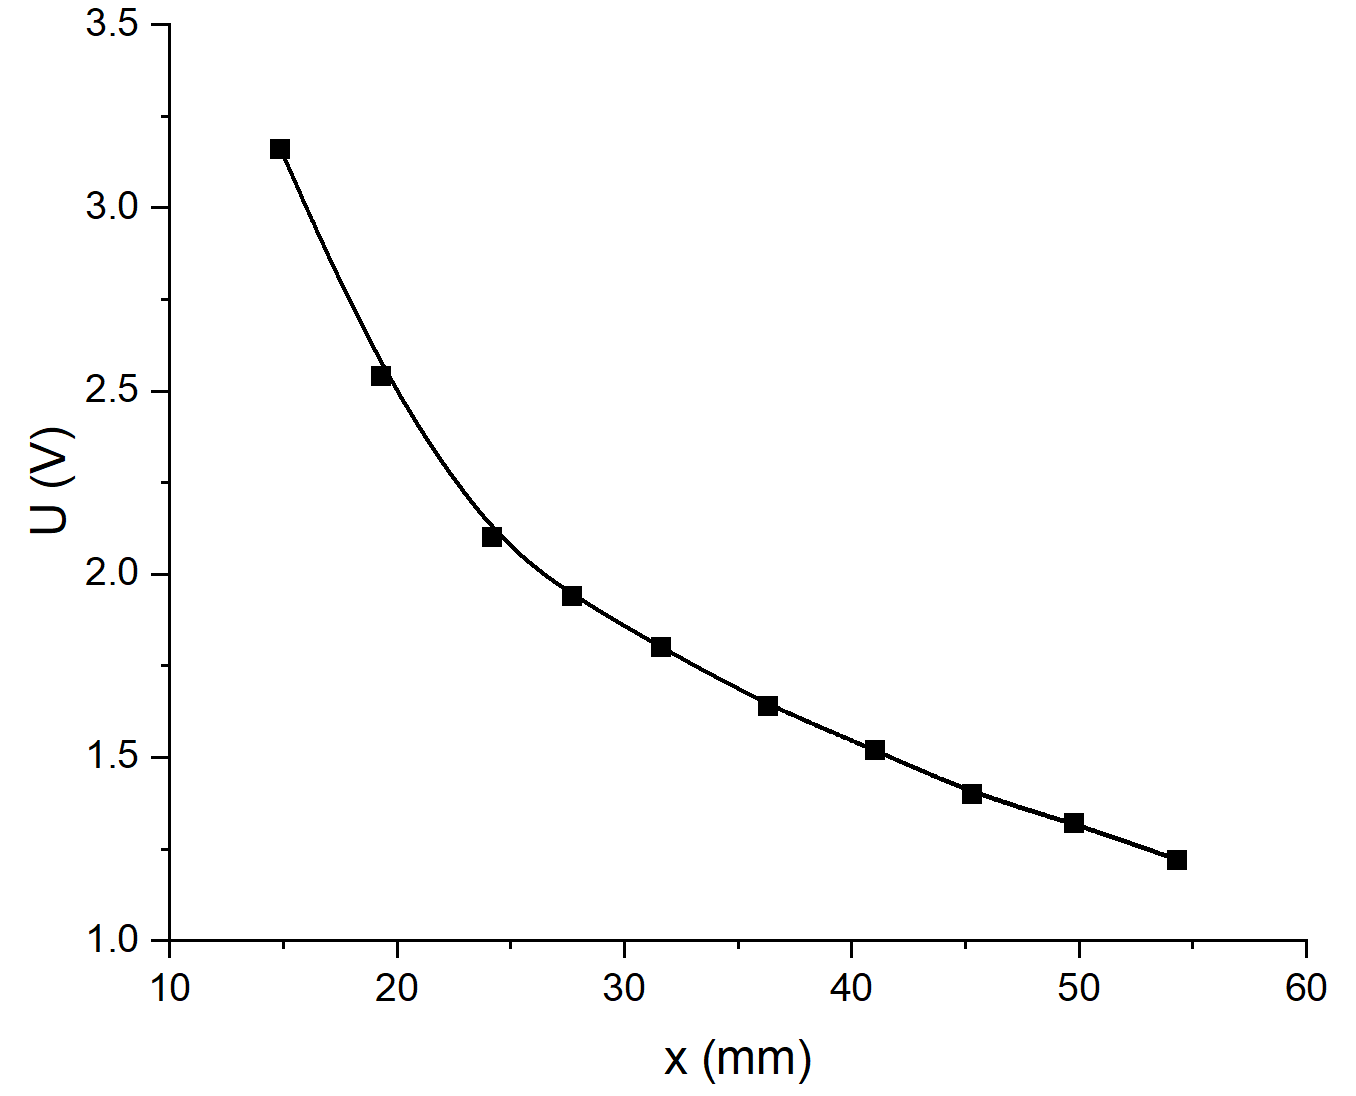
\includegraphics[width=8cm]{fig1.png}
		\caption{电压峰峰值与位置的关系}
	\end{figure}
	由图可知,电压峰峰值衰减速度随距离增加而变慢,图像类似于e指数衰减的图像。
	\section{原始数据}
	\begin{figure}[H]
		\centering
		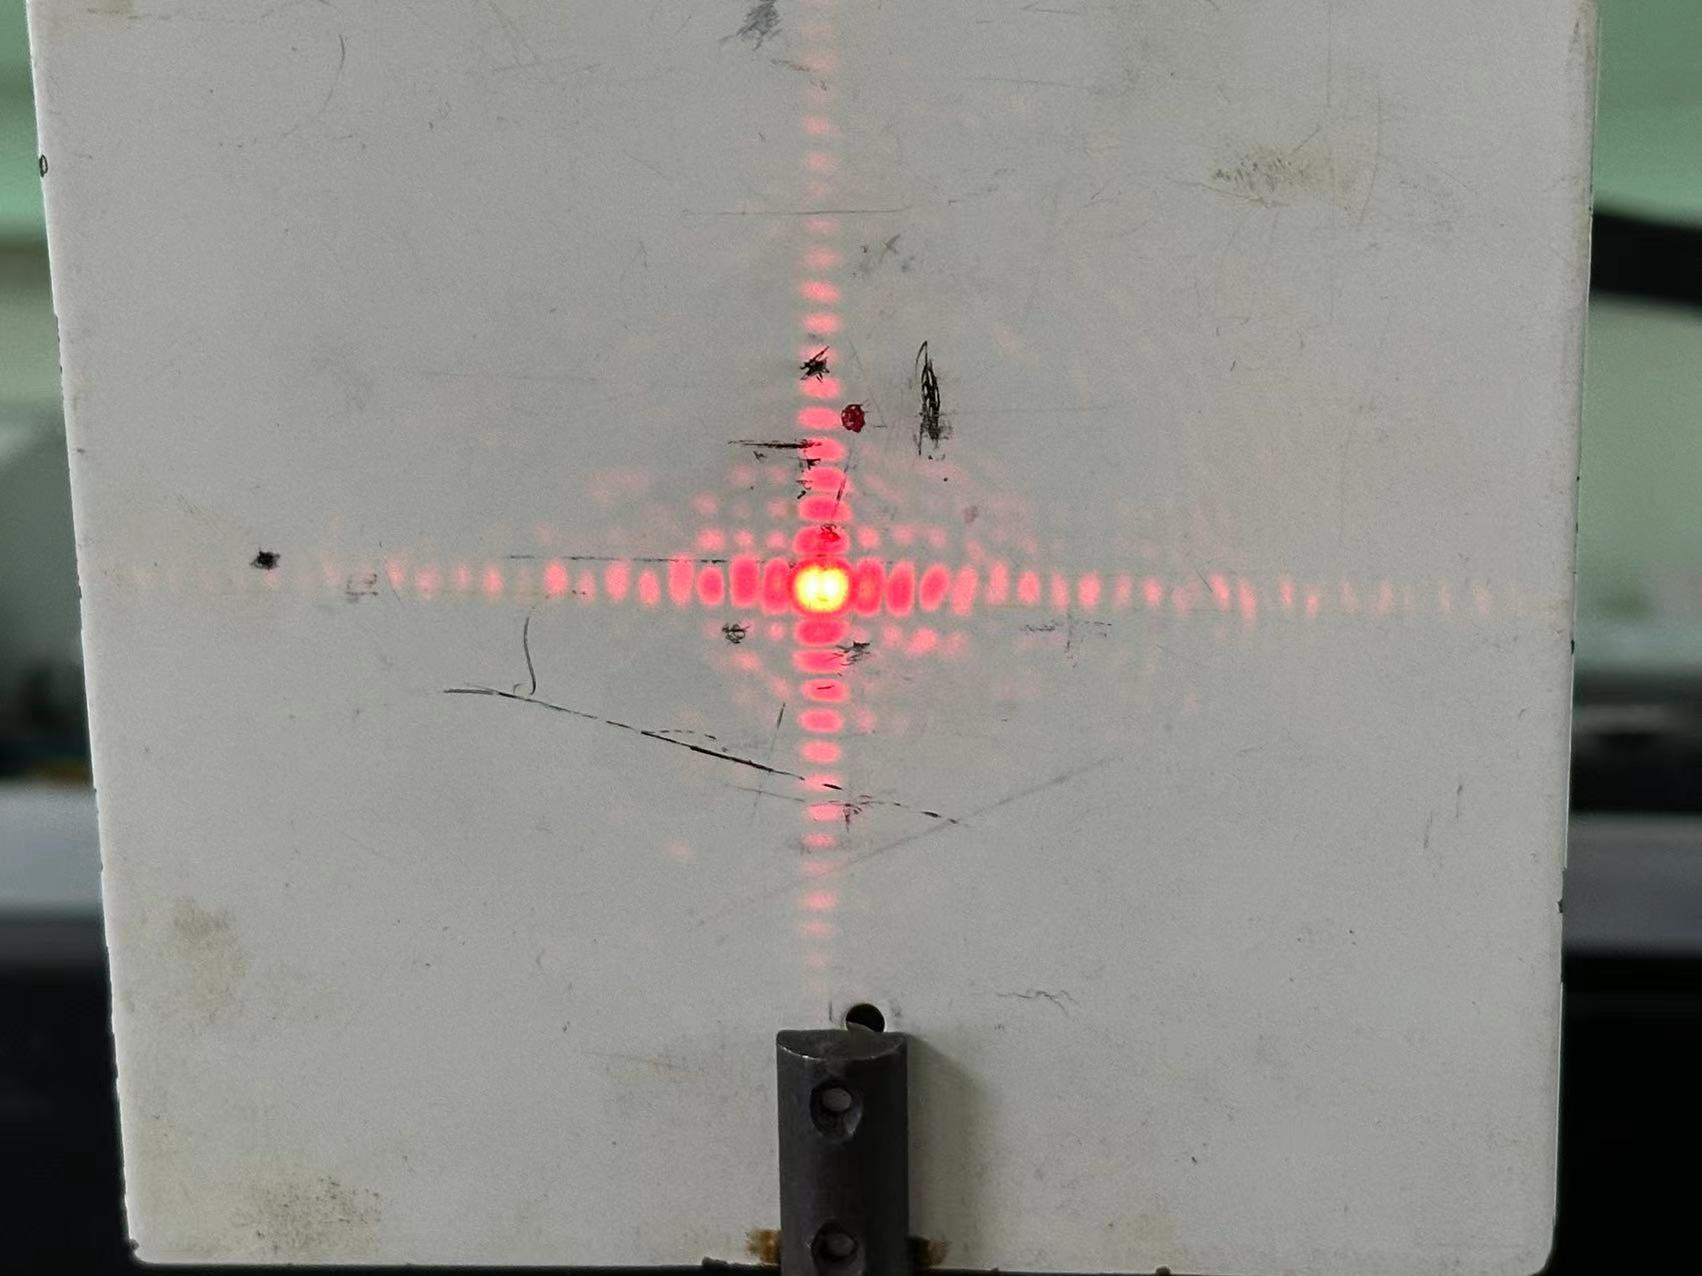
\includegraphics[width=15cm]{1.jpg}
	\end{figure}
	\begin{figure}[H]
	\centering
	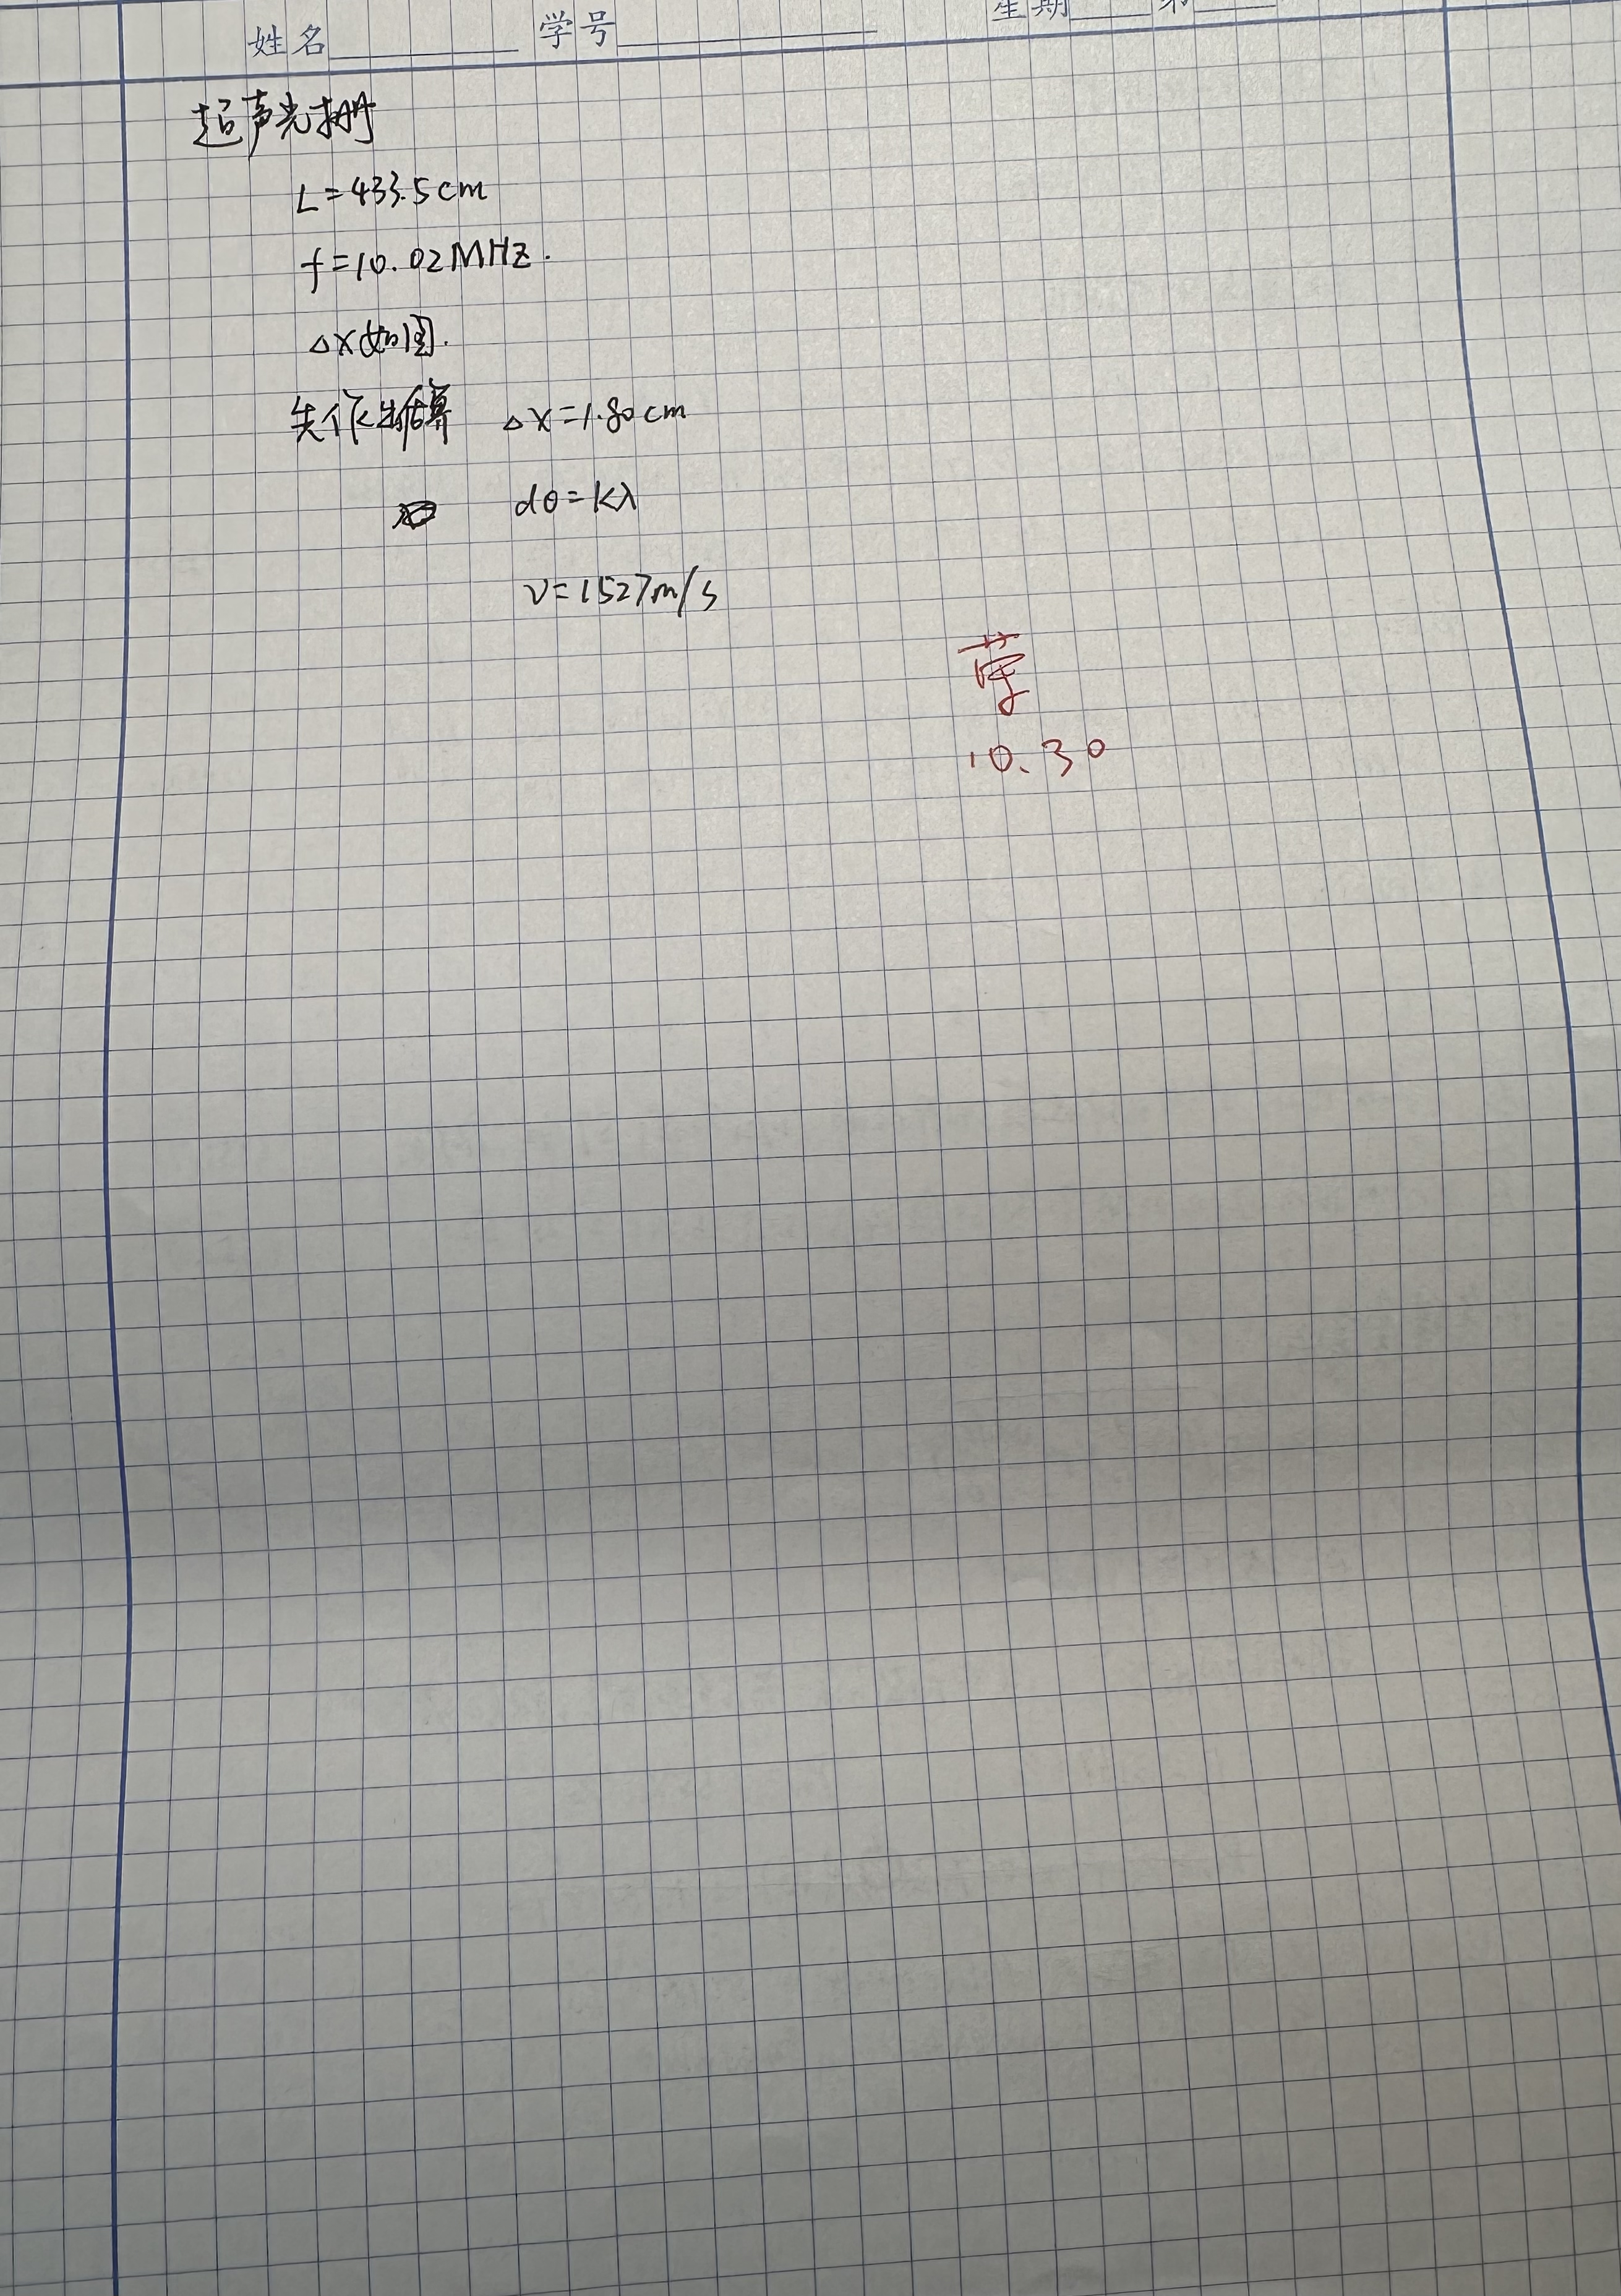
\includegraphics[width=15cm]{2.jpg}
	\end{figure}
	\begin{figure}[H]
	\centering
	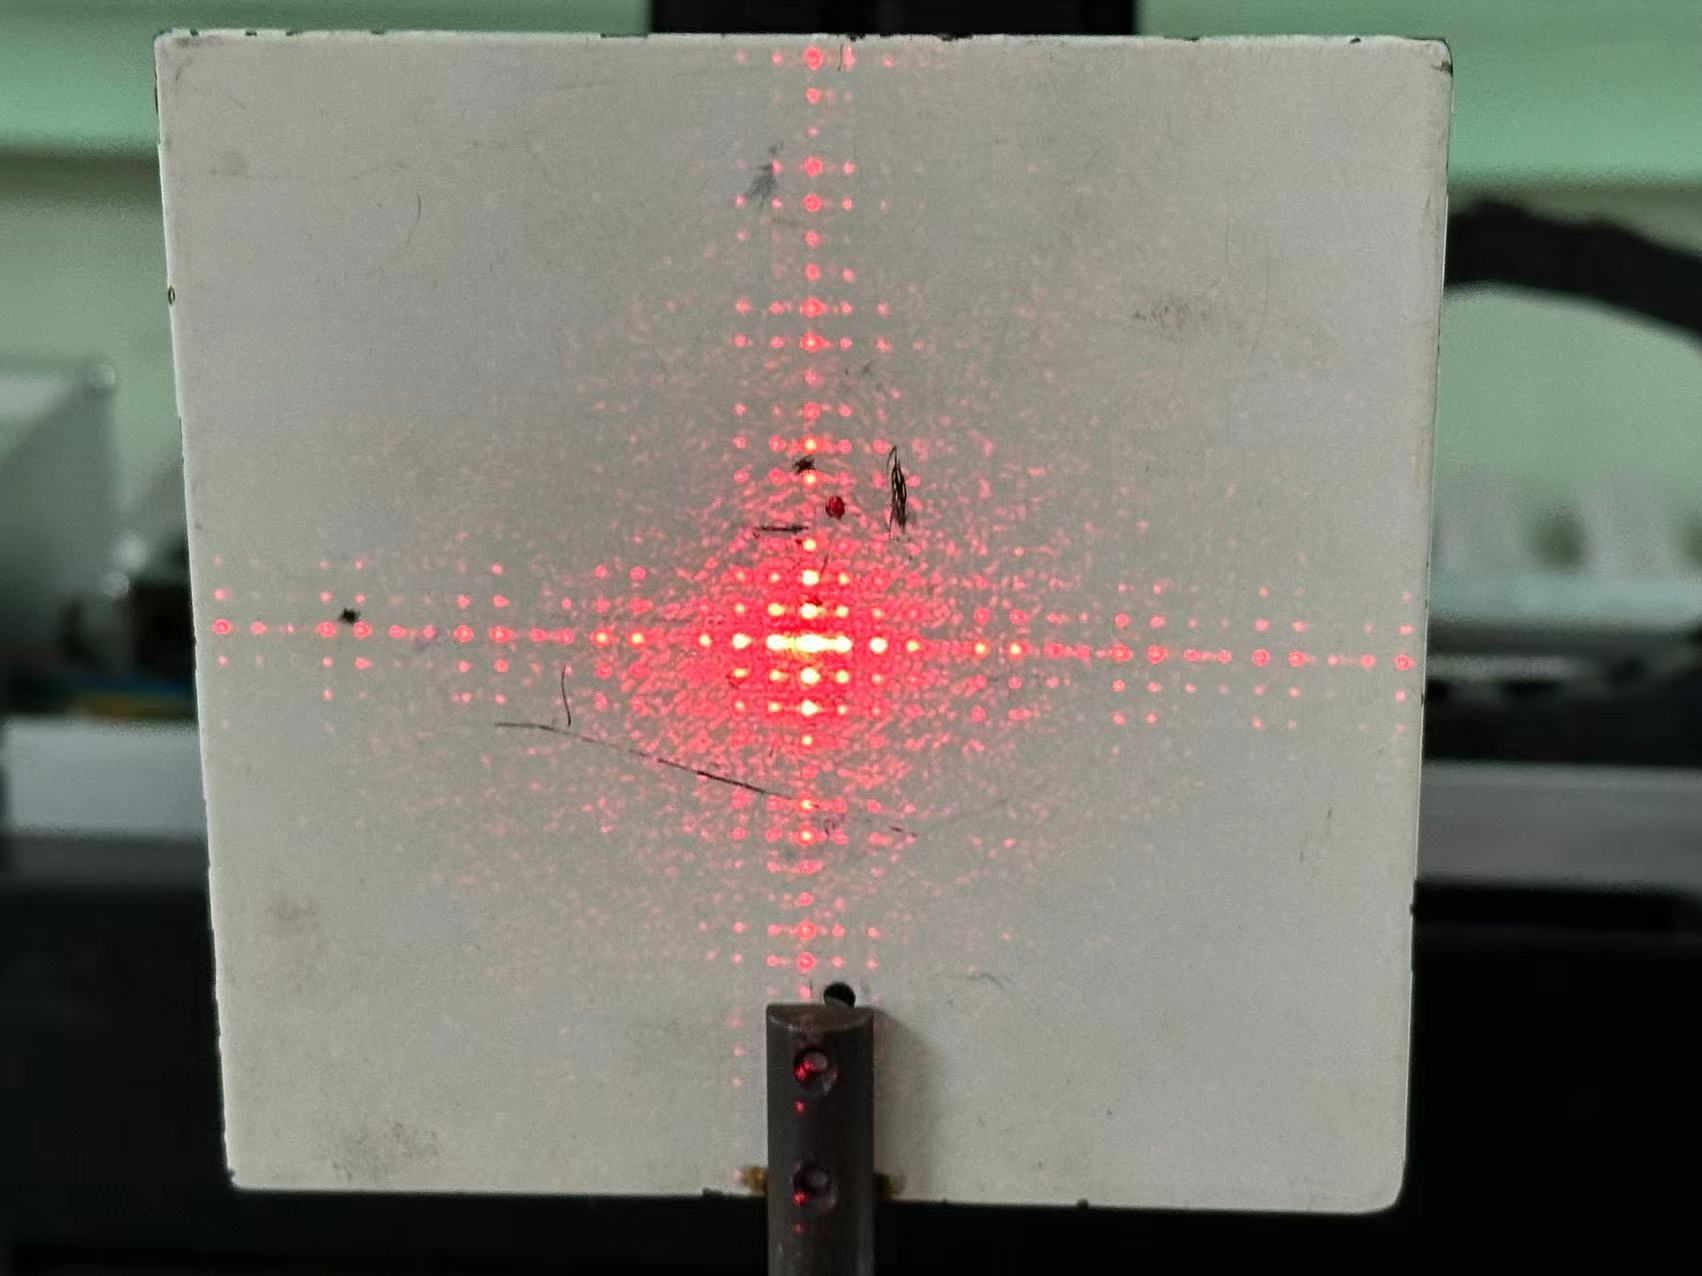
\includegraphics[width=15cm]{3.jpg}
	\end{figure}
\end{document}